\documentclass[12pt,a4paper,headsepline]{scrreprt}

\usepackage{ucs}
\usepackage[utf8x]{inputenc}
\usepackage[T1]{fontenc}
\usepackage[ngerman]{babel}
\usepackage{blindtext}
\usepackage{scrlayer-scrpage}
\usepackage{graphicx}
% \usepackage{footnote}
\usepackage{amsfonts}
\usepackage{amsmath}
\usepackage[onehalfspacing]{setspace}
\usepackage[
	left=2.6cm,
	right=2.8cm,
	top=2.5cm,
	bottom=2.5cm
			]{geometry}
%\newgeometry{
%  left=3cm,
%  right=3cm,
%  top=2.5cm,
%  bottom=2.5cm,
%  bindingoffset=0mm
%}
% Listoffigures, Listoftables, Listofindex werden in Toc angezeigt
% \usepackage{tocbibind}

% Moderne Schriftart wird verwendet
\usepackage{lmodern}
\usepackage{textcomp} %bestimmte sonderzeichen
\newcommand{\eur}[1]{\mbox{#1\,\texteuro}\xspace}
% Tabellen ---------------------------------------------------------------------
\PassOptionsToPackage{table}{xcolor}
\usepackage{tabularx}
% für lange Tabellen
\usepackage{longtable}
\usepackage{array}
\usepackage{ragged2e}

% pdfs einbinden
\usepackage{pdfpages}

\usepackage{lscape}
\newcolumntype{w}[1]{>{\raggedleft\hspace{0pt}}p{#1}}
\usepackage{xcolor}
\usepackage{url}
% Tabellen-, Equation- und Figurenummerierung ist nicht Chapter gebunden
\usepackage{chngcntr}
\counterwithout{table}{chapter}
\counterwithout{equation}{chapter}
\counterwithout{figure}{chapter}
% Tabellen werden nicht nach Chapter nummeriert
\renewcommand{\thetable}{\arabic{table}}

% Abstand zwischen Nummerierung und Überschrift definieren
% > Schön wäre hier die dynamische Berechnung des Abstandes in Abhängigkeit
% > der Verschachtelungstiefe des Inhaltsverzeichnisses
\newcommand{\headingSpace}{1.5cm}
% Für die Einrückung wird das Paket tocloft benötigt
\usepackage[titles]{tocloft}
%\cftsetindents{chapter}{0.0cm}{\headingSpace}
%\cftsetindents{section}{0.0cm}{\headingSpace}
%\cftsetindents{subsection}{0.0cm}{\headingSpace}
%\cftsetindents{subsubsection}{0.0cm}{\headingSpace}
%\cftsetindents{figure}{0.0cm}{\headingSpace}
%\cftsetindents{table}{0.0cm}{\headingSpace}

\setlength{\parindent}{0em}
\usepackage{makeidx}
\usepackage{varioref}
\usepackage{hyperref}
\hypersetup{%
  linktocpage 	= true,
  colorlinks  	= true,
  linkcolor   	= blue,
}

% Tabellenfärbung:
\definecolor{heading}{RGB}{100,165,245}
%\definecolor{heading}{rgb}{0.64,0.78,0.86}
\definecolor{odd}{rgb}{0.9,0.9,0.9}

% fügt Tabellen aus einer TEX-Datei ein
\newcommand{\tabelle}[3]{
\begin{table}[htbp]
\centering
\singlespacing
\input{#3}
\caption{#1}
\label{#2}
\end{table}}

\newcommand{\Anhang}[1]{\appendixname{}~unter~\ref{#1}: \nameref{#1}}
\newcommand{\tab}[1]{Tabelle~\ref{#1}~\nameref{#1}}
\newcommand{\sectionref}[1]{\ref{#1}~\nameref{#1}}
\newcommand{\bildref}[1]{\ref{#1}~\nameref{#1}}
\renewcommand{\thetable}{\arabic{table}}

\automark{chapter}
\automark*{section}
\clearpairofpagestyles
%\ihead{\headmark}
%\ihead{\footnotesize Migration und Modifikation der autoritativen DNS-Infrastruktur \\mit der Implementierung von DNSSEC}
%\ohead{\includegraphics[scale=0.047]{Bilder/logo_interchalet.png} }
\ifoot{Viktor Gange - Mt. 4924109}
\ofoot{\pagemark}
\renewcommand*\chapterpagestyle{scrheadings} 	% Die erste Chapter Seite bekommt auf die
												% Weise auch einen Header

\begin{document}
\pagenumbering{arabic}


% Inhalt
\section*{Plots}
\begin{center}


\begin{tikzpicture}
\begin{axis}[
	title={Lineares Sondieren},
    enlargelimits=false,
    xlabel={Größe des Hashtables},
    ylabel={Zeit [ms]}
]
\addplot+[
    scatter]
table[meta=x]
{lineareSondieren.dat};
\end{axis}
\end{tikzpicture}

\end{center}
\vspace*{3mm}

\begin{center}
\begin{tikzpicture}
\begin{axis}[
	title={Lineares Sondieren, random},
    enlargelimits=false,
    xlabel={Größe des Hashtables},
    ylabel={Zeit [ms]}
]
\addplot+[
    scatter]
table[meta=x]
{lineareSondierenRandom.dat};
\end{axis}
\end{tikzpicture}
\end{center}
\clearpage

\begin{center}
\begin{tikzpicture}
\begin{axis}[
	title={Doppel Hashing},
    enlargelimits=false,
    xlabel={Größe des Hashtables},
    ylabel={Zeit [ms]}
]
\addplot+[
    scatter]
table[meta=x]
{doppelHashing.dat};
\end{axis}
\end{tikzpicture}
\end{center}

\begin{center}
\begin{tikzpicture}
\begin{axis}[
	title={Doppel Hashing, random},
    enlargelimits=false,
    xlabel={Größe des Hashtables},
    ylabel={Zeit [ms]}
]
\addplot+[
    scatter]
table[meta=x]
{doppelHashingRandom.dat};
\end{axis}
\end{tikzpicture}
\end{center}
\clearpage

\subsection*{Aufgabe 2}
\textbf{a)}\\
Die Erste for Schleife geht von $i=1$ bis $n-1$ durch das Array A.\\
Die Zweite for Schleife geht von $j=0$ bis $i-1$ ebenfalls durch das Array A.\\
Die Dritte for Schleife geht von $k=0$ bis $n-1$ ebenfalls durch das Array A.\\
Dabei wird jeweils die Absolute Differenz von dem Element A[i] und dem Element A[j] mit dem Element A[z] verglichen und falls die gleich sind wird ein True zurückgegeben, und falls alle Schleifen durchlaufen und die If-Bedingung kein einziges mal zutrifft wird ein False zurückgegeben.\\

Die asymptotische Laufzeit beträgt:~~~ $\mathcal{O}((n-1)(n-1)n) = \mathcal{O}(n^3)$\\

\textbf{b)}\\
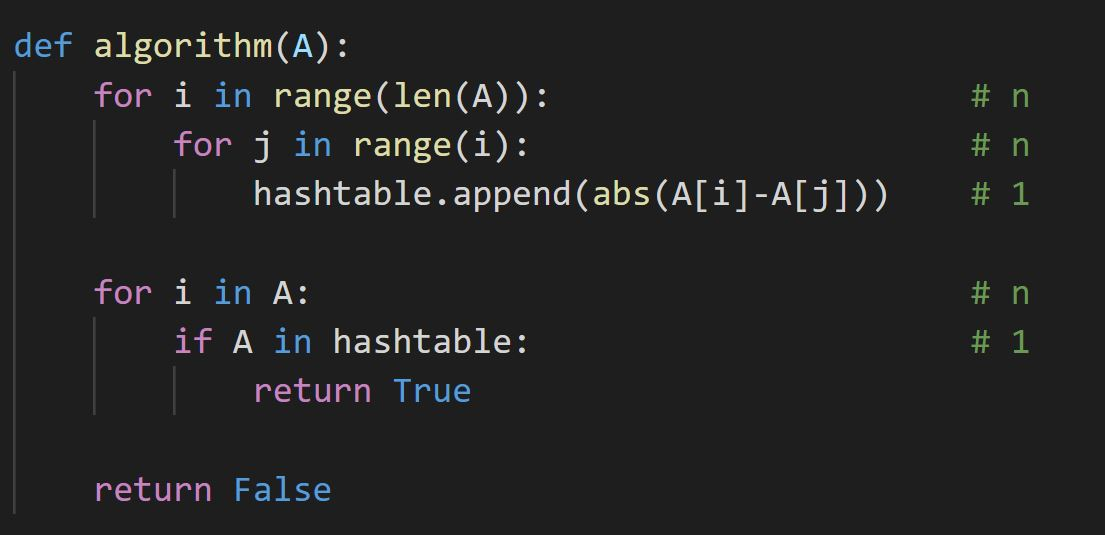
\includegraphics[scale=0.8]{2b.jpg}\\

Wie man an dem Pseudocode sieht, können wir mit Hashtables die Hintereinanderreihung von for Schleifen auf 2 statt 3 begrenzen, dadurch haben wir ein asymptotische Laufzeit von:~~~ $\mathcal{O}(n*n + n) ~=~ \mathcal{O}(n^2)$
\clearpage

\textbf{c)}\\
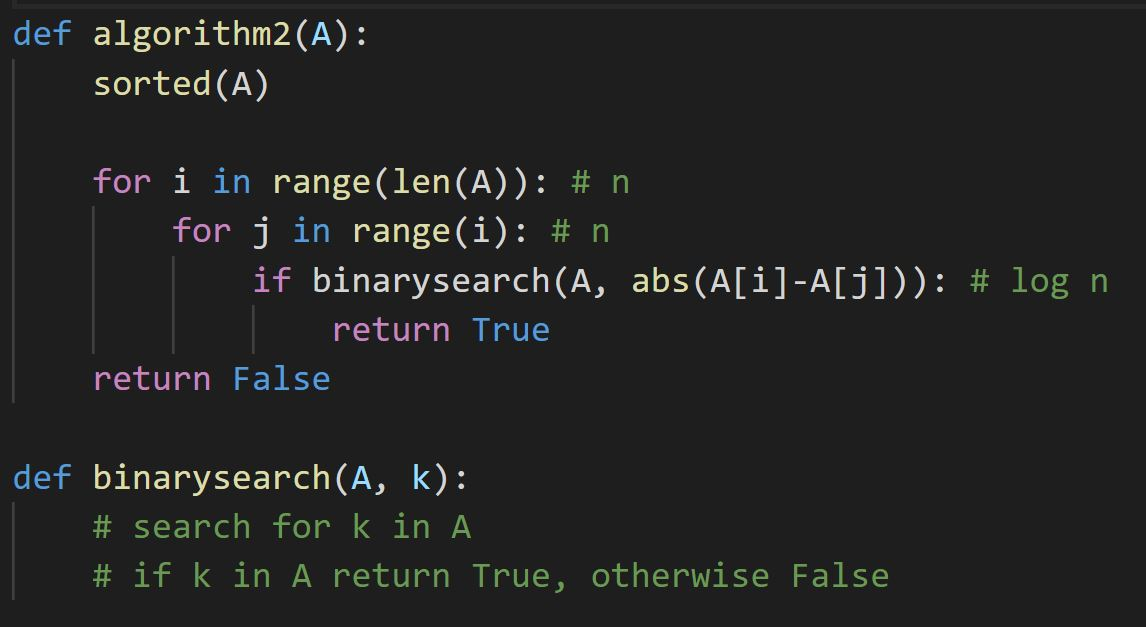
\includegraphics[scale=0.77]{2c.jpg}\\

Wie man an dem Pseudocode sieht, sortieren wir zuerst das Array A.\\
Wie auch bei b beschränken wir uns hier auf zwei for Schleifen, das ist möglich weil wir eine sortierte Liste und den Binary Search verwenden, welches nur eine Laufzeit von $\mathcal{O}(\log n)$ hat.\\
Die asymptotische Laufzeit insgesamt beträgt also:~~~ $\mathcal{O}(n*n*\log n) ~=~ \mathcal{O}(n^2 \log n)$




 

\end{document}
